\documentclass[sigconf]{acmart}

\usepackage{booktabs} % For formal tables
\usepackage{float}
\usepackage{arydshln} % for dashed lines in tables (tabu is much more flexible)
\usepackage{enumitem}
\newcommand{\ra}[1]{\renewcommand{\arraystretch}{#1}} %array spacing
\usepackage{natbib}
\usepackage{graphicx}
\graphicspath{{data/}}
\frenchspacing % controls the space after the period
\usepackage{pdfpages}
\usepackage{nicefrac}
\usepackage{blindtext}
\usepackage{tabularx}
\usepackage{caption}
\captionsetup[table]{font=small,skip=4pt}
\captionsetup[figure]{font=small,skip=-2pt}
\usepackage{subcaption}
\usepackage{bm} % produces better bold symbols than does \boldsymbol{x}; use \bm{x}
\usepackage{amsmath, mathrsfs,amsfonts,amssymb}
\usepackage{wasysym} % smiley face
\usepackage{xfrac} % use command \sfrac{1}{2} to get a nice 1/2 symbol.
\usepackage{savesym} % openbox symbol conflict between tx fonts and amsthm
\savesymbol{openbox}
\usepackage{amsthm} %theorem like environments
\usepackage{thmtools}
\usepackage{cleveref}
\usepackage{commath}
\usepackage[export]{adjustbox}
\usepackage{dblfloatfix}
\usepackage{tikz}
\usepackage{blindtext}
\usepackage{xcolor}
\usepackage{url}
\usetikzlibrary{backgrounds}

\definecolor{lightgray}{HTML}{989898}
\definecolor{darkgray}{HTML}{696969}

\newcommand{\lightgraybg}[1]{%
  \begingroup\setlength{\fboxsep}{3pt}% no padding
  \raisebox{2pt}{\colorbox{lightgray}{#1}}
  \endgroup
}

\newcommand{\darkgraybg}[1]{%
  \begingroup\setlength{\fboxsep}{3pt}% no padding
  \raisebox{2pt}{\colorbox{darkgray}{#1}}
  \endgroup
}

\newcommand{\psame}{p_{\scriptsize\mbox{same}}}
\newcommand{\pdiff}{p_{\scriptsize\mbox{diff}}}
\newcommand{\pjump}{p_{\scriptsize\mbox{jump}}}
\newcommand{\pout}{p_{\scriptsize\mbox{out}}}
\newcommand{\plink}{p_{\scriptsize\mbox{link}}}
\newcommand{\rlocal}{r_{\scriptsize\mbox{local}}}

\crefname{subsection}{subsection}{subsections}

\newcommand{\hs}[1]{\textcolor{red}{Hari: #1}}
\newcommand{\harshay}[1]{\textcolor{blue}{Harshay: #1}}

% Copyright
\setcopyright{none}

% DOI
% \acmDOI{10.475/123_4}
% \acmISBN{123-4567-24-567/08/06}
% \acmConference[CIKM'17]{ACM CIKM}{Nov 2017}{Singapore }
\acmYear{2018}
\copyrightyear{2016}
\settopmatter{printacmref=false} % Removes citation information below abstract
\renewcommand\footnotetextcopyrightpermission[1]{} % removes footnote with conference information in first column
\pagestyle{plain}

\begin{document}
\title{Growing Attributed Networks through Local Processes}

% \author{Harshay Shah, Suhansanu Kumar, Hari Sundaram}
% \affiliation{
%   \institution{
%   Department of Computer Science \\
%   University of Illinois at Urbana-Champaign}
% }
% \email{{hrshah4, skumar56, hs1}@illinois.edu}

% \renewcommand{\shortauthors}{Anonymous et al.}

\begin{abstract}
%!TEX root = ../main.tex

This paper proposes an attributed network growth model. Despite the knowledge
that individuals use limited resources to form connections to similar others, we
lack an understanding of how local and resource-constrained mechanisms explain
the emergence of rich structural properties found in real-world networks. We
make three contributions. First, we propose an interpretable and accurate model
of attributed network growth that jointly explains the emergence of in-degree
distribution, local clustering, clustering-degree relationship and attribute
mixing patterns. Second, we make use of biased random walks to develop a model
that forms edges locally, without recourse to global information. Third, we
account for multiple sociological phenomena: bounded rationality; structural
constraints; triadic closure; attribute homophily; preferential attachment.
% We explore the parameter space of the proposed Attributed Network Growth (\texttt{ARW})
% to show each model parameter intuitively modulates network structure.
Our experiments show that the proposed Attributed Network Growth (\texttt{ARW}) model
accurately preserves network structure and attribute mixing patterns of
six real-world networks; it improves upon the performance of eight
well-known models by a significant margin of
2.5--$10\times$.

\end{abstract}

% \keywords{Network growth models, Attributed networks, Homophily}

\maketitle

%!TEX root = draft.tex

\section{Introduction}
\label{sec:Introduction}


% what is the problem?

We develop a resource constrained model of network growth that explains the
emergence of key structural properties. The problem is important for several
reasons. Individuals form real-world networks acting under resource constraints
and while using local information. These networks that individuals form exhibit
rich structural properties. However, we lack an understanding of mechanisms that
are resource constrained and which use local information explain the emergence
of these structural related properties.

% why is it important?

Classic models of network growth, make unrealistic assumptions about what agents
who form edges do. Consider as a simple stylized example, the process of finding
the a set of papers to cite when writing an article. In the preferential
attachment model \cite{barabasi1999emergence} of network growth, a node making
$m$ citations would pick a paper uniformly at random from \textit{all} papers in
the domain, and either cite it or copy one of its references. We would repeat
this process, till we've exhausted our budget of $m$ references. Notice that the
process assumes access to the entire dataset, and that one would pick papers
uniformly at random. An equivalent formulation of this copying model
is to cite papers from the entire dataset in proportion to their in degree. The
latter formulation assumes that agent making citations know the entire in-degree
distribution. While preferential attachment models explains the emergence of
the power-law degree distribution, the attachment model is an unrealistic
representation of how agents make decisions on edge formation.

%why is it hard?

The problem of developing a model of network growth, where agents act under
resource constraints, including access to only local information is hard. The
problem lies in identifying simple mechanisms, with few parameters, where the
agents only use local information and \textit{jointly} preserve the properties
related structure.

% what did we do?

We propose a random walk based model of network growth that jointly explains the
emergence of the following properties: heavy-tailed in-degree distributions,
local clustering and clustering-degree relationships. In the growth model, an
incoming node picks a recent node as the seed. It will link to this node with
some constant linking probability. Then, it follows the outgoing link or the
incoming link of this seed node and arrives at a new node. At each new node, it
decides to link with the same constant linking probability. Then it has to
decide whether to jump back to the seed node, or following incoming or outgoing
links. The process repeats until the agent has exhausted its budget for linking.
To summarize, new nodes concurrently acquire information and form edges
by exploring the local neighborhoods of existing nodes, without access to the
entire network.

\begin{figure}[t]
 \centering
 \includegraphics[width=\columnwidth]{intro_plot3}
 \caption{
 }
 \label{fig:intro_plot}
\end{figure}


Our main contributions are as follows:
\begin{itemize}
    \item We propose a model
    of network growth using a local edge formation mechanism that incorporates the
    resource constraints that influence individuals' edge formation mechanisms in
    real-world networks.
    \item We propose a model that jointly explains multiple
    structural properties, including in-degree distribution, clustering, degree
    clustering relationship and edge densification.
\end{itemize}


We conducted extensive experimental results, against state of the art
baselines, on large citation network datasets. We show that our growth model
outperforms that best competing model in jointly and accurately preserving
multiple structural properties---degree distribution, clustering and
degree-clustering relationship---by a significant margin.

The rest of the paper is organized as follows. In~\Cref{sec:Related Work}, we
describe the related work. Then, in~\Cref{sec:Preliminaries}, we define key
structural properties and introduce the datasets. We formally state the goal of
the paper in~\Cref{sec:Problem Statement}. In~\Cref{sec:Empirical Analysis}
and~\Cref{sec:Proposed Model}, we report prominent structural characteristics
of citation networks and propose a network growth model respectively. This is
followed by~\Cref{sec:Experiments}, where we validate our model against
multiple baselines.


\begin{table*}
 {
  \begin{tabular}[c]{llrrrc|rrrr} \toprule
   Network &  Description & $|V|$           & $|E|$        & $T$        & $A$, $|A|$  &  \texttt{LN} $(\mu, \sigma)$ & \texttt{DPL} $\alpha$       &  Avg. ${\texttt{LCC}}$  & \texttt{AA} $r$           \\ \midrule
   \texttt{USSC}~\cite{fowler2008authority}  & U.S. Supreme Court cases         & 30,288     & 216,738      & 1754-2002  & -   & (1.19, 1.18) & 2.32     & 0.12    & -     \\
   \texttt{HEP-PH}~\cite{gehrke2003overview} & ArXiv Physics manuscripts     & 34,546     & 421,533      & 1992-2002  & -  &   (1.32, 1.41) & 1.67     & 0.12    & -                 \\
   \texttt{Semantic}~\cite{ammar}&   Academic Search Engine  & 7,706,506  & 59,079,055   & 1991-2016  & -   &   (1.78, 0.96)  & 1.58     & 0.06    & -             \\   \midrule
   \texttt{ACL}~\cite{acldata}    & NLP papers      & 18,665     & 115,311      & 1965-2016  & \textsc{venue}, 50  &   (1.93, 1.38)  & 1.43     & 0.07    & 0.07  \\
   \texttt{APS}~\cite{aps}     & Physics journals     & 577,046    & 6,967,873    & 1893-2015  & \textsc{journal}, 13 &   (1.62, 1.20)  & 1.26     & 0.11    & 0.44 \\
   \texttt{Patents}~\cite{leskovec2005graphs}   & U.S. NBER patents    & 3,923,922  & 16,522,438   & 1975-1999  & \textsc{category}, 6 &   (1.10, 1.01)   & 1.94     & 0.04    & 0.72 \\
   % \texttt{PYPI}         & 25,169     & 71,371       & 2002-2018  & \textsc{category} & 9  \\
  \bottomrule
  \end{tabular}
  \vspace{1mm}
  \caption{Summary statistics \& global properties of six network datasets: $|V|$ nodes join the networks and form edges $|E|$ over
  time period $T$. In attributed networks, each node has a categorical attribute value that belongs to set $A$ of size $|A|$.
  The networks exhibit lognormal (\texttt{LN}) in-degree distribution with mean $\mu$ and standard deviation $\sigma$,
  high average local clustering (${\texttt{LCC}}$) \& attribute assortativity (\texttt{AA}) coefficient and
  densify over time with power law (\texttt{DPL}) exponent $\alpha$.}
  \label{table:datasets}
  \label{table:netstats}
 }
\end{table*}


%!TEX root = draft.tex

\section{Problem Statement}
\label{sec:Problem Statement}

Consider an attributed directed network $G=(V,E,B)$, where $V$ \& $E$ are
sets of nodes \& edges and each node has an attribute value $b \in B$.
The goal is to develop a directed network growth model that preserves structural
and attribute based properties observed in $G$. The growth model should be
normative, accurate and parsimonious:
\begin{enumerate}
    \item \textbf{Normative}: The model should account for normative behavior. In real-world
    networks, multiple sociological phenomena influence how individuals form edges under
    constraints of limited global information and partial network access.
    \item \textbf{Accurate}: The model should preserve key structural
    and attribute based properties such as heavy tailed degree distribution, skewed
    local clustering, negatively correlated degree-clustering relationship
    and attribute mixing patterns.
    \item \textbf{Parsimonious}: The model should have as few parameters as possible, but be expressive enough to generate networks with varying structural properties.
\end{enumerate}

Next, we present empirical analysis on real-world datasets to motivate our attributed random walk model.





% \clearpage
%!TEX root = ../main.tex

\section{Empirical Analysis}
\label{sec:Analysis}

We first describe six large-scale network datasets.
Then, we describe global network properties,
insights from empirical studies and common assumptions in
network modeling.

\subsection{Datasets}
\label{sec:Datasets}

We consider six citation networks of different scales (size, time) from diverse
sources: research articles, utility patents and judicial cases. ~\Cref{table:datasets} lists their
summary statistics and global network properties.  Three of the six datasets are attributed networks;
that is, each node has a categorical attribute value.

We focus on citation networks for two reasons. First, since nodes in citation networks form
all outgoing edges to existing nodes at the time of joining the network,
these datasets provide a clean basis to study edge formation in
attributed networks. Second, the node-level, temporal information in datasets that span long time periods (e.g. \texttt{USSC})
enables us to study structural properties at different time stages via network snapshots.
Next, we study the structural and attribute properties of these networks.

\subsection{Global Network Properties}
\label{subsec:factors}

Statistical descriptors of network properties ~\cite{newman2010networks}
such as degree distribution, local clustering, and attribute assortativity
quantify the extent to which edge formation shapes global network
structure.

\textbf{Degree distribution:}
Real-world networks tend to exhibit heavy tailed degree distributions in which
a small but significant fraction of the nodes turn into high-degree hubs.
We observe that Log-normal fits, with parameters listed in~\Cref{table:netstats}, well describe
the in-degree distributions, consistent with Broido and
Clauset's~\cite{broido2018scale} observation that scale-free, real-world networks
are rare.

\begin{figure}
 % \vspace{-10pt}
 \centering
 \includegraphics[width=\columnwidth]{clustering}
 \caption{
    Real-world networks exhibit
    skewed local clustering distribution (left subplot) and a negatively correlated
    relationship between in-degree and average local clustering (right subplot).
 }
 \label{fig:cc_dc}
 % \vspace{-10pt}
\end{figure}

\textbf{Local Clustering:}
Real-world networks exhibit high local clustering
(\texttt{LCC}), as shown in~\Cref{table:netstats}. Local
clustering can arise from triadic closure~\cite{simmel1950sociology,
newman2001clustering}, where nodes with common neighbor(s) have an increased
likelihood of forming a connection.
The coefficient of node $i$ equals the probability with which two randomly chosen
neighbors of the node $i$ are connected. In directed networks, the neighborhood
of a node $i$ can refer to the nodes that link to $i$, nodes that
$i$ links to or both. We define the neighborhood to be the set
of all nodes that link to node $i$. In ~\Cref{fig:cc_dc}, we show that (a) average local clustering is not a
representative statistic of the skewed local clustering distributions and (b) real-world networks
exhibit a negative correlation between in-degree and clustering.
That is, low in-degree nodes have small, tightly knit neighborhoods
and high in-degree nodes tend have large, star-shaped neighborhoods.


% Homophily and Assortativity
\textbf{Homophily:}
Attributed networks tend to exhibit homophily~\cite{mcpherson2001birds}, the
phenomenon where similar nodes are more likely to be connected than dissimilar
nodes. The assortativity coefficient ~\cite{newman2002assortative} $r \in [-1,
1]$, quantifies the level of homophily in an attributed network.
Intuitively,
assortativity compares the observed fraction of edges between nodes with the same attribute
value to the expected fraction of edges between nodes with same attribute value
if the edges were rewired randomly. In~\Cref{fig:mixing}, we show that
attributed networks \texttt{ACL}, \texttt{APS} and \texttt{Patents} exhibit
varying level of homophily with assortativity coefficient ranging from $0.07$ to
$0.72$.


\begin{figure}
 \centering
 \includegraphics[width=\columnwidth]{homophily}
 \caption{
    Attributed networks \texttt{ACL}, \texttt{APS} and \texttt{Patents} exhibit
    homophily w.r.t attributes \texttt{Venue} ($r=0.07$), \texttt{Journal} ($r=0.44$) and
    \texttt{Category} ($r=0.72$) respectively.
 }
 \label{fig:mixing}
 \vspace{-20pt}
\end{figure}



\textbf{Increasing Out-degree over Time:}
The out-degree of nodes that join real-world networks tends to increase as
functions of network size and time. This phenomenon densifies networks and
can shrink effective diameter over time. Densification tends to exhibit a power law
relationship ~\cite{leskovec2005graphs} between the number of edges $e(t)$ and
nodes $n(t)$ at time $t$: $e(t) \propto n(t)^{\alpha}$.~\Cref{table:netstats}
lists the densification power law (\texttt{DPL}) exponent $\alpha$ of the
network datasets.

To summarize, citation networks tend to be homophilic networks that undergo
accelerated network growth and exhibit regularities in structural properties:
heavy tailed in-degree distribution, skewed local clustering distribution,
negatively correlated degree-clustering relationship, and varying attribute
mixing patterns.

\subsection{Insights from Sociological Studies}

Sociological studies on network formation seek to explain
how individuals form edges in real-world networks.

\textbf{Interplay of Triadic Closure and Homophily:}
Empirical studies~\cite{35626,block2014multidimensional} that analyze the
interplay between triadic closure and homophily
 % in evolving networks
  indicate
that \textit{both} structural proximity and homophily are statistically
significant factors that simultaneously influence edge formation.
Homophilic preferences~\cite{mcpherson2001birds} induce edges between similar
nodes, whereas structural factors such as network distance limit
edge formation to proximate nodes (e.g. friend of a
friend).

\textbf{Bounded Rationality:}
Extensive work~\cite{simon1972theories,gigerenzer1996reasoning,lipman1995information} on
decision making shows that individuals are boundedly rational
actors; constraints such as limited information, cognitive capacity and time impact decision making.
This suggests that resource-constrained individuals that join networks are likely to employ simple rules
to form edges using limited information and partial network access.


Current preferential attachment and fitness-based models
\cite{dorogovtsev2000structure,singh2017relay,barabasi1999emergence}
make two assumptions that are at variance with these findings.
First, by assuming that successive edge formations are independent,
these models disregard the effect of triadic closure and structural proximity.
Second, as discussed in~\cref{sec:Introduction}, these models require complete network
access or knowledge of node-level properties.

Insights from sociological studies indicate that edge formation in real-world
networks comprises biases towards nodes that are similar, well-connected or
structurally proximate. Coupled with empirical analyses, it also motivates
the need to model how resource-constrained edge formation processes collectively
shape global network properties of large-scale networks over time.


% \clearpage
%!TEX root = draft.tex

\section{Attributed Random Walk Model}
\label{sec:Proposed Model}
The Attributed Random Walk (\texttt{ARW}) model explains the emergence
of key structural properties of real networks through local edge formation mechanisms.
First, we describe the edge formation mechanisms underlying \texttt{ARW}. Then,
we briefly discuss the methods required to fit the model to data.


\subsection{Model Description}
\label{sub:Model Description}

\texttt{ARW} grows a directed network over time as new nodes join the network.
The mechanism that nodes use to form edges intuitively corresponds to how we
expect researchers to conduct a literature survey and cite relevant work.
First, the researcher broadly identifies \textit{relevant} papers,
possibly with the help of external information sources.
Then, under time and information constraints, the individual navigates a chain
of references to identify \textit{similar} papers that either support or
address the problem in hand.  Next, through careful analysis, he or she
decides to cite a subset of these papers; Heuristics such as number of
citations maybe used in the decision making process.
Incoming nodes in \texttt{ARW} use a similar mechanism to form edges.
New nodes select a seed node and initiate a random walk to (a) explore the network
by navigating through neighborhoods of existing nodes and (b) probabilistically
link to visited nodes based on attribute similarity, as shown in \Cref{fig:randomwalk}.

The Attributed Random Walk (\texttt{ARW}) model grows a directed network $\{G_t\}^T_{t=1}$.
More formally, at every discrete time step $t$, a
new node $u$, with attribute value $A(u)$, joins the network $G_t=(V_t, E_t,
A_t)$, where $V_t, E_t$ and $A_t$ are sets of nodes, edges and unique attribute
values at time $t$. After joining the network, node $u$ forms $m(t)$ edges to
existing nodes. At time $t$, $G_t$ consists of ${|V_t|=|V_0|+t}$ nodes,
${|E_t|=|E_{t-1}|+m(t)}$ edges and the set of attribute values ${A_t = A_{t-1}
\cup \{A(u)\}}$.
% Outdegree $m(t)$ of incoming nodes increases over time to
% reflect the nonlinear growth and densification of real networks.
We discuss the
issue of initializing $G_0$, sampling attribute value $A(u)$ and modeling
densification using $m(t)$ in \Cref{sub:Model Fitting}.

The edge formation mechanism consists of two components: \textsc{Select-Seed} and
\textsc{Random-Walk}. A new node $u$ with attribute value $A(u)$ that joins the
network at time $t$ first selects a seed node $s_u$ using \textsc{Select-Seed}:
\\\\
\tikzstyle{background rectangle}=[thin,draw=black]
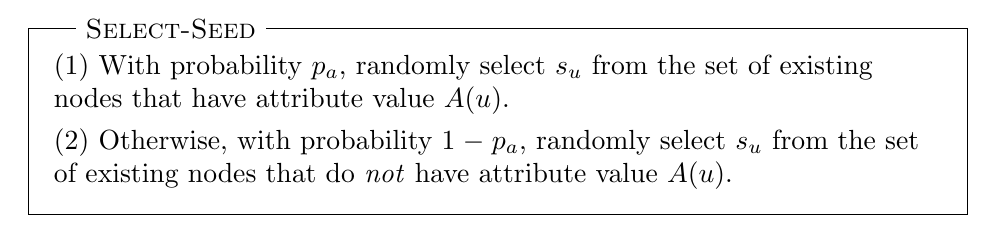
\begin{tikzpicture}[show background rectangle]
\node[align=left, text width=.93\linewidth, inner sep=.5em]{
(1) With probability $p_a$, randomly select $s_u$ from the set of existing nodes that have attribute
value $A(u)$.

\vspace{1mm}
(2) Otherwise, with probability $1-p_a$, randomly select $s_u$ from the set of existing nodes that
do \textit{not} have attribute value $A(u)$.
};
\node[xshift=3ex, yshift=-.7ex, overlay, fill=white, draw=white, above
right] at (current bounding box.north west) {
\textsc{Select-Seed}
};
\end{tikzpicture}

% The attribute parameter $p_a$ incorporates the attribute preferences of incoming nodes
% into the model.
In \textsc{Seed-Select}, attribute parameter $p_a$ is the probability with which
an incoming node and its seed node have the same attribute value.
% As shown in \Cref{fig:randomwalk}, node $u$ has homophilic preferences if $p_a$ is greater than the fraction of existing nodes with attribute value $A(u)$.
After selecting the seed $s_u$, node $u$ initiates a random walk using
\textsc{Random-Walk} to form $m(t)$ links:
\\\\
\tikzstyle{background rectangle}=[thin,draw=black]
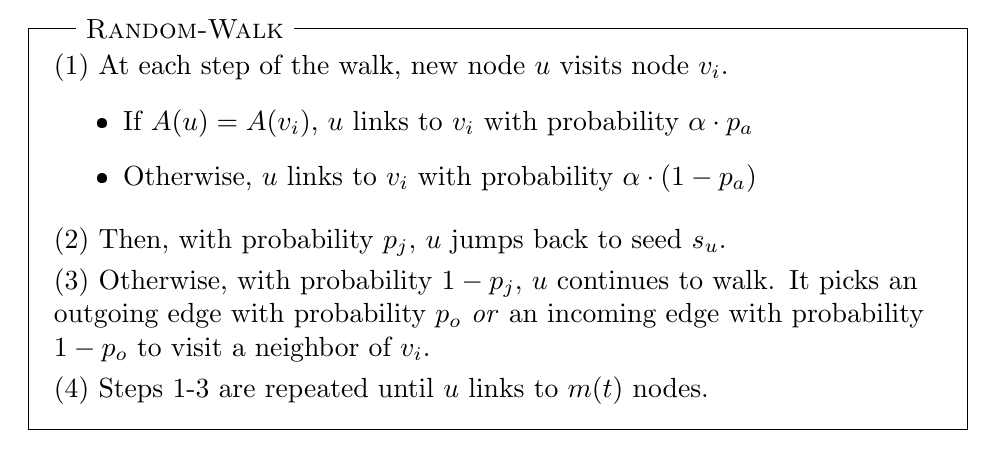
\begin{tikzpicture}[show background rectangle]
\node[align=left, text width=.93\linewidth, inner sep=.5em]{
(1) At each step of the walk, new node $u$ visits node $v_i$.
    \begin{itemize}
        \item If $A(u)=A(v_i)$, $u$ links to $v_i$ with probability $\alpha \cdot p_a$
        \item Otherwise, $u$ links to $v_i$ with probability $\alpha \cdot (1-p_a)$
    \end{itemize}

\vspace{1mm}
(2) Then, with probability $p_j$, $u$ jumps back to seed $s_u$.

\vspace{1mm}
(3) Otherwise, with probability ${1-p_j}$, $u$ continues to walk. It picks an outgoing edge with probability $p_o$ \textit{or}
an incoming edge with probability $1-p_o$ to visit a neighbor of $v_i$.

\vspace{1mm}
(4) Steps 1-3 are repeated until $u$ links to $m(t)$ nodes.
};
\node[xshift=3ex, yshift=-.7ex, overlay, fill=white, draw=white, above
right] at (current bounding box.north west) {
\textsc{Random-Walk}
};
\end{tikzpicture}

Random walks inherently account for limited information and partial network access as
they only require information about the neighborhood of visited nodes.
\begin{figure}[h]
    \centering
    \includegraphics[width=.9\linewidth]{random_walk}
    \vspace{3mm}
    \caption{Edge formation in \texttt{ARW}.
    A new node $u$ joins the attributed network with outdegree ${m=3}$ and attribute value
    {$A(u)=\textsc{red} \in \{\textsc{red},\textsc{blue}\}$}.
    It uses \textsc{Select-Seed} to select seed node $v_a$ and initiates a \textsc{Random-Walk}.
    As denoted by the labeled edges, node $u$ starts from $v_a$, moves to $v_b$, jumps back to seed $v_a$ and
    visits $v_c, v_d, v_e$ and $v_f$. It links to three nodes ---  $v_b$, $v_d$ \& $v_f$ ---
    that have the same attribute value.}
    \label{fig:randomwalk}
    \vspace{-2mm}
\end{figure}

The \textsc{Random-Walk}
mechanism consists of four parameters - $\alpha$ \& $p_a$
parameterize edge formation decisions and $p_j$ \& $p_o$ characterize random walk
traversals:
\begin{itemize}
    \item The rate parameter $\alpha$ controls the rate at which $u$ links to
    visited nodes; It implicitly incorporates triadic closure because the
    probability that node $u$ ``closes'' a triad by linking to an existing node
    $v_i$ and its neighbors is proportional to $\alpha^2$.

    \item The attribute parameter $p_a$ accounts
    for homophily/heterophily by incorporating attribute preferences of incoming nodes
    into the model.

    \item The jump parameter $p_j$ is the probability with which $u$ restarts the
    random walk from seed $s_u$; It controls the extent to which structural constraints restrict $u$ to link to nodes that are
    structurally proximate and in the same locality.

    \item The out parameter $p_o$ is the probability with which a node chooses an
    outgoing edge in its random walk traversal. Incoming nodes can visit old nodes
    by randomly traversing the network using \textit{outgoing} edges because an
    edge from $u$ to $v$ exists iff $u$ joins the network after $v$. Moreover,
    random walk models \cite{vazquez2000knowing} exhibit positive correlation between node
    indegree and node age observed in real networks.
    As a result, $p_o$ incorporates bias towards high
    degree nodes by controlling the rate at which incoming nodes approach old nodes.
\end{itemize}

In the absence of attribute data, the edge formation mechanisms are further simplified
because the attribute parameter $p_a$ is not required. \textsc{Seed-Select} simplifies
to selecting an existing node uniformly at random and edge formation in \textsc{Random-Walk}
depends on the rate parameter $\alpha$ only.

To summarize, the Attributed Random Walk (\texttt{ARW}) model
intuitively describes how individuals form edges under resource constraints.
\texttt{ARW} uses four parameters --- $\alpha$, $p_a$, $p_j$, $p_o$ --- to incorporate
individuals' biases towards similar, proximate and high degree nodes.

\subsection{Model Fitting}
\label{sub:Model Fitting}
We now briefly describe methods to estimate \texttt{ARW} parameters,
initialize $\hat{G}$ at time ${t=0}$, densify $\hat{G}$
over time and sample incoming nodes' attribute values.

\textit{Parameter Estimation}.
The rate parameter $\alpha$, attribute parameter $p_a$, jump parameter $p_j$ and
out parameter $p_o$ jointly control the edge formation mechanism in \texttt{ARW}.
These parameters subsequently determine the structural properties of the network $\hat{G}$
generated by \texttt{ARW}. The parameter estimation task consists of finding the set of
parameters values for $(\alpha, p_a, p_j, p_o)$ that best explain the structural properties
of an observed network $G=(V,E,A)$. We use a straightforward grid search method to estimate
the four parameters. We describe the evaluation metrics and selection criteria in \Cref{sub:Experimental Setup}.
Other derivative-free optimization methods such as the Nelder-Mead method can be used to quicken parameter estimation.

\textit{Initialization}. The edge formation mechanism in \texttt{ARW} is
sensitive to a large number of weakly connected components \texttt{WCC}s in the
initial network $\hat{G}_0$ because incoming nodes can only form edges to nodes
in the same \texttt{WCC}. To ensure that $\hat{G}_0$ is weakly
connected, we perform an undirected breadth-first search on the observed,
to-be-fitted network $G$ that starts from the oldest node and terminates after
visiting $0.1$-$1\%$ of the nodes. The initial network $\hat{G}_0$ is the small
subgraph induced from the set of visited nodes.
% Simpler initialization methods
% such as sampling $\hat{G}_0$ from the Erdos-Renyi model or Watts-Strogatz model
% yield similar results.

\textit{Densification}. In \cref{sec:Analysis}, we observed that real
networks densify over time, with the number of edges growing superlinearly in
the number of nodes. We incorporate densification into \texttt{ARW} by
increasing the outdegree of new nodes that \textit{sequentially} join the
network $\hat{G}$.
Each incoming node $u$ that joins $\hat{G}$ at time $t$ corresponds to some
 node that joins the observed network $G$ in
year $y(t)$; The number of edges $m(t)$ that $u$ forms is equal to the average
outdegree of nodes that join $G$ in year $y(t)$. Therefore, the rate of growth
in $\hat{G}$ coarsely reflects the rate of growth in $G$.

\textit{Sampling Attribute Values}. In real networks $G=(V,E,A)$,
the distribution over the set of attribute values $P_{\textsc{g}}(A)$ changes over time.
For instance, the attribute distribution over journals in the \texttt{APS} citation
network changes over time as old journals decay in popularity and new journals gain traction.
To incorporate this phenomenon into \texttt{ARW}, we sample the attribute value $A(u)$ of node $u$, that
joins $\hat{G}$ at time $t$, from $P_{\textsc{g}}(A{\mbox{ | year}=y(t)})$, the observed attribute distribution
conditioned on the corresponding year of node $u$.


In this section, we described the Attributed Random Walk
model and discussed methods related to model fitting. Next, our experiments in
\cref{sec:Experiments} show that $\texttt{ARW}$ accurately preserves
\textit{multiple} structural properties of real networks
% \Cref{sec:Experiments}, we show that the cumulative effect of the edge
% formation processes in \texttt{ARW} --- triadic closure, strong homophily,
% structural constraints and preferential attachment --- explains the emergence
% of high clustering, assortative mixing and heavy tailed degree distributions in
% real networks.

% The goal of our resource-constrained
% model is to generate networks that follow structural properties of real networks
% discussed in~\Cref{sec:Empirical Analysis}.
% Third, we show that
% \texttt{ARW} intrinsically incorporates local processes --- preferential
% attachment, triadic closure and homophily --- that effect edge formation in real
% networks.

% \subsection{Empirical Observations}
% \label{sub:Empirical Observations}
%
% \texttt{ARW} grows a directed network over time as new nodes join the network.
% The mechanism that nodes use to form edges intuitively corresponds to how we
% expect researchers to conduct a literature survey and cite relevant work.
% First, the researcher broadly identifies \textit{relevant} papers.
% possibly with the help of external information sources.
% Then, under time and information constraints, the individual navigates a chain
% of references to identify \textit{similar} papers that either support or
% address the problem in hand.  Next, through careful analysis, he or she
% decides to cite a subset of these papers; Heuristics such as number of
% citations maybe used in the decision making process.
%
% Incoming nodes in \texttt{ARW} use a similar mechanism to form edges.
% New nodes select a seed node and initiate a random walk to (a) explore the network
% by navigating through neighborhoods of existing nodes and (b) probabilistically
% link to visited nodes based on attribute similarity, as shown in \Cref{fig:randomwalk}.
% The following observations guide the development of the Attributed Random Walk model.
% \vspace{-2mm}
% \begin{enumerate}
%     \item \textbf{Proximity \& homophily}: Sociological studies \cite{35626,block2014multidimensional,mcpherson2001birds} on
%     evolving social networks indicate that both, structural proximity and
%     homophily, are important factors that influence edge formation. Homophilic
%     preferences cause similarity-induced edge formation whereas structural
%     factors act as constraints that restrict opportunities to structurally proximate
%     nodes (e.g. friend of a friend).
%
%     \item \textbf{Biased human navigation}: Analysis \cite{west2012human} of Wikispeedia \cite{west2009wikispeedia},
%      a game in which players must navigate from page \texttt{X} to page
%     \texttt{Y} using as few hyperlinks as possible, sheds light on how individuals
%     navigate networks with limited, \textit{local} information. Their
%     findings indicate that individuals (a) move to well-connected, high-degree pages
%     that maximize information and (b) rely on pages' content attributes to reach \texttt{Y}.
%
%     \item \textbf{Decision making under constraints}: Individuals make edge
%     formation decisions based on limited information and
%     partial network access.
%     For example, a researcher cites references without
%     knowing or having access to all papers in her field.
% \end{enumerate}
%
%
% Based on these observations, an edge formation mechanism should account for bias
% towards nodes that are similar, proximate or well-connected. It should also
% incorporate resource constraints to model how individuals form
% edges in real networks.
% % Nodes in \texttt{ARW} use random walks to
% % explore the network and link to existing nodes concurrently.
% % Random walk traversals only require information about the neighborhood of a small subset of visited nodes.
% Next, we describe the edge formation mechanism in \texttt{ARW}.


% \subsection{Parameter Space}
% \label{sub:Parameter Space}
%
% In this subsection, we study the variability in the structural properties of
% networks generated by our model. We also show that each model parameter
% is necessary because it influences different aspects of global network
% structure.



% \clearpage
%!TEX root = ../draft.tex

\begin{figure*}[t]
	\vspace{-15pt}
	\centering
	\makebox[\textwidth][c]{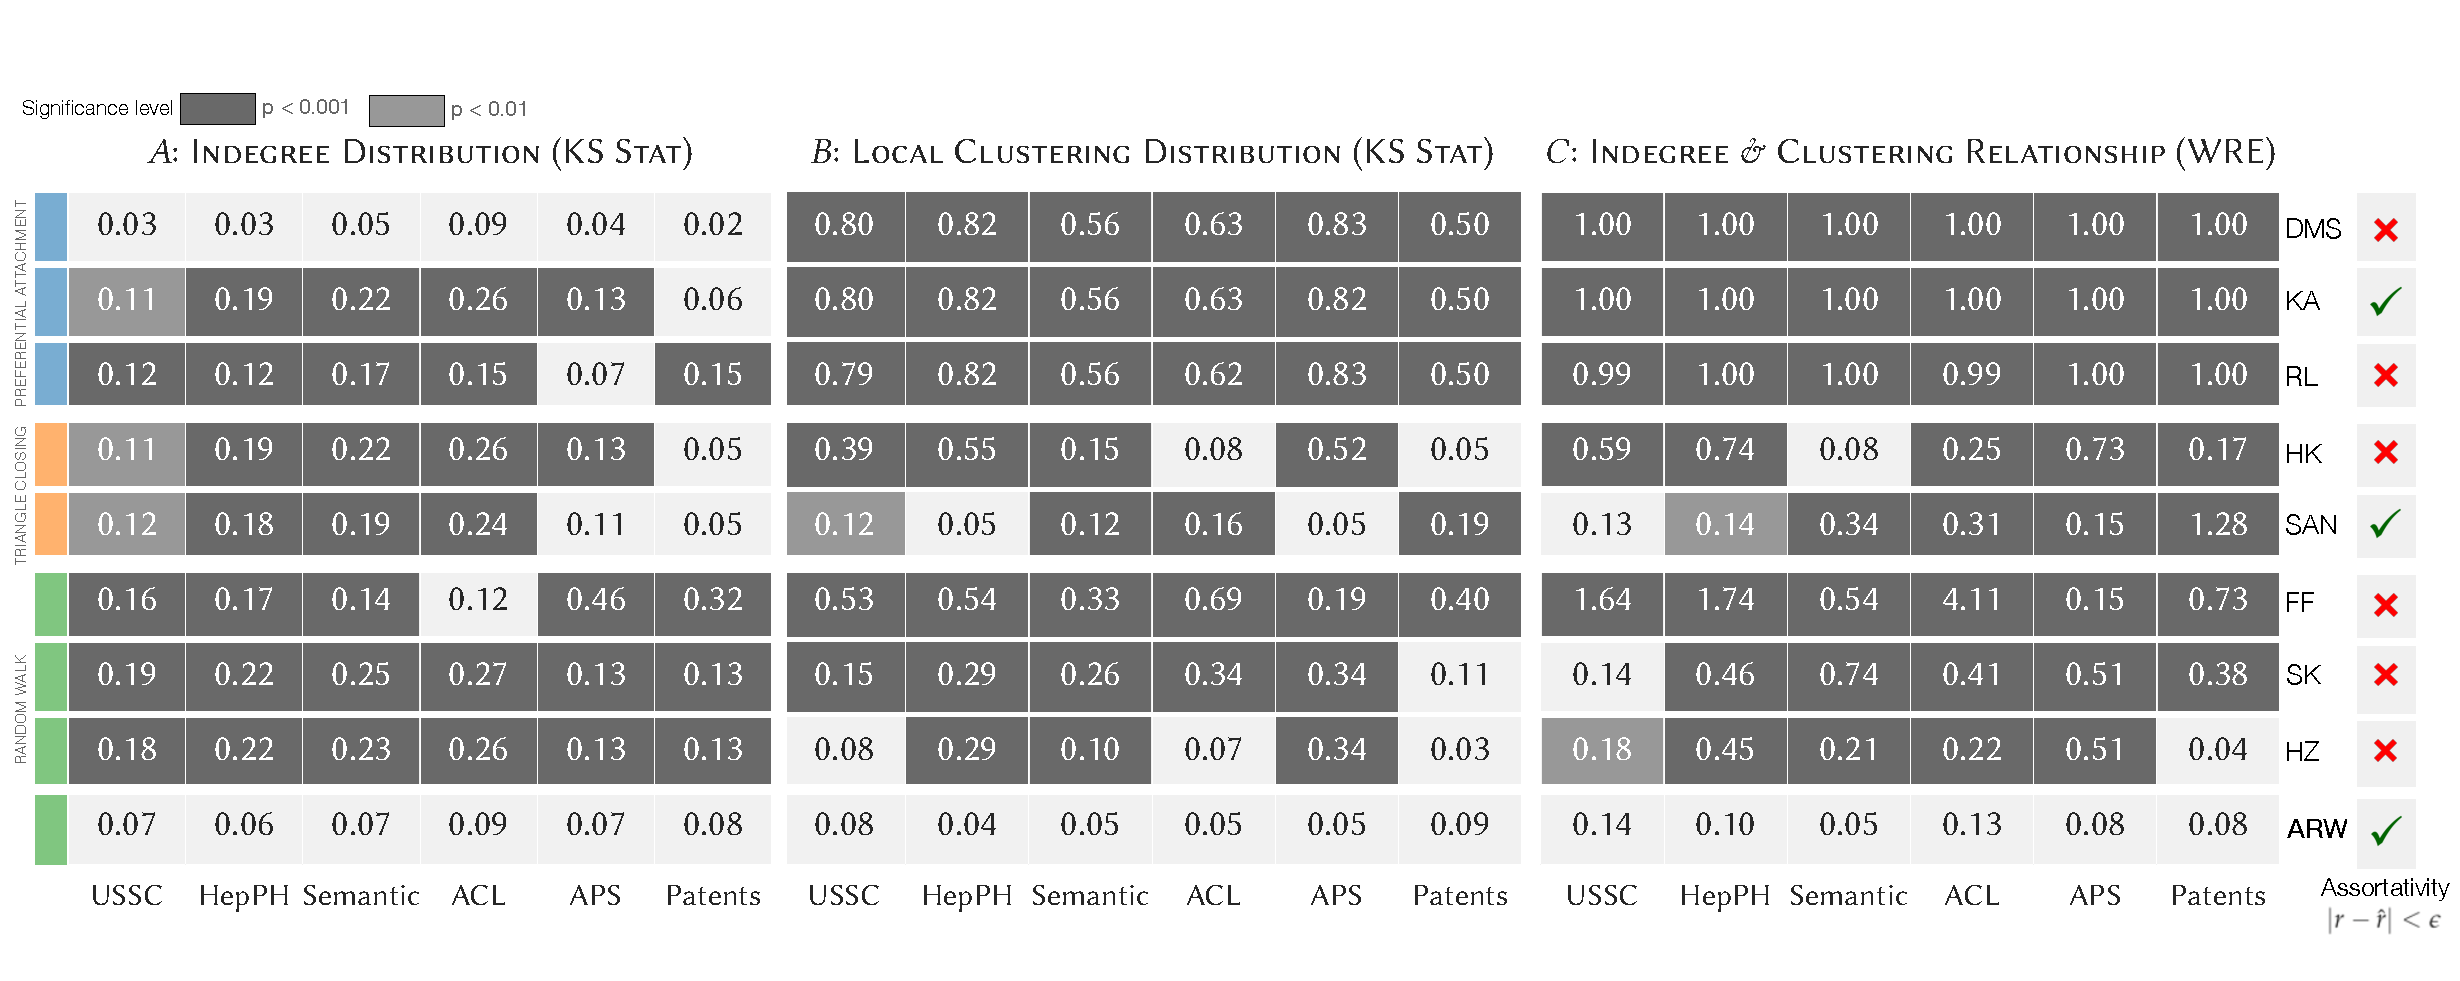
\includegraphics[width=\textwidth]{experiments}}
	\vspace{-16pt}
	\caption{
		Modeling network structure. We assess the extent to which network models
		fit key structural properties of six real-world networks. Tables 5A, 5B and 5C
		measure the accuracy of eight models in fitting the in-degree distribution,
		local clustering distribution, in-degree \& clustering relationship
		respectively and global attribute assortativity.
		Existing models tend to underperform because they either disregard
		the effect of factors such as triadic closure and/or homophily
		or are unable to generate networks with varying structural properties.
		Our model, \texttt{ARW}, jointly preserves all three properties accurately and often
		performs considerably better than existing models:
		the cells are shaded gray or dark gray if the proposed model \texttt{ARW} performs
		better at significance level $\alpha=0.01$ ( \lightgraybg{ }) or $\alpha=0.001$ ( \darkgraybg{ })
		respectively.
		%  Models with green \checkmark fit the assortativity
		% coefficient of attributed networks ---\texttt{ACL}, \texttt{APS} and
		% \texttt{Patents}--- up to 2 decimal places.
		% % We group models based on their
		% underlying edge formation mechanisms: preferential attachment, triangle closing
		% or random walks.
		% properties based on clustering. Models equipped with triangle closing
		% mechanisms ---\texttt{HK}, \texttt{SAN}---are not flexible enough to
		% accurately fit the skewed local clustering distributions of real-world
		% networks. Existing random walk models \texttt{FF}, \texttt{SK} and
		% \texttt{HZ} perform poorly because they are not expressive enough to
		% generate networks with varying structural properties.
	}
	\vspace{-10pt}
	\label{fig:exp_table}
\end{figure*}

\section{Modeling Network Structure}
\label{sec:Experiments}
In this section, we evaluate the effectiveness of \texttt{ARW} in preserving
structural properties of network datasets described in~\Cref{sec:Datasets}.
relative to eight state-of-the-art growth models.
% In~\Cref{sub:Experimental Setup}, we begin by describing existing growth models and the evaluation metrics
% used in the experiments. Then, we discuss our results.

\subsection{Setup}
\label{sub:Experimental Setup}

% We first briefly summarize the existing models used in the experiments.
In this subsection, we describe the state-of-the-art, representative growth models
and evaluation metrics used to fit these growth models to network datasets.

\textit{State-of-the-art Growth Models}. We compare \texttt{ARW} to eight state-of-the-art
growth models representative of the key edge formation
mechanisms: preferential attachment, fitness, triangle closing and random walks.
Two of the eight models account for attribute homophily and preserve attribute mixing patterns,
as listed below:
\begin{enumerate}
	\item{\textbf{Dorogovtsev-Mendes-Samukhin model}} \cite{dorogovtsev2000structure}  (\texttt{DMS})
	is a preferential attachment model that generates directed scale-free graphs. In this model,
	the probability of linking to a node is proportional to the sum of its in-degree and ``initial attractiveness.''

	\item{\textbf{Relay Linking model}} \cite{singh2017relay} (\texttt{RL}) propose a set of
	preferential attachment models for directed networks, which use relay linking to explain the change in
	node popularity over time. We use the iterated preferential relay-cite (IPRC) variant, which best fits
	real-world network properties.

	\item{\textbf{Kim-Altmann model}} \cite{kim2017effect} (\texttt{KA}) is a fitness-based model that defines
	fitness as the product of degree and attribute similarity. It can generate \textit{attributed} networks
	with assortative mixing and heavy tailed degree distribution.
	To generate directed networks, we modify \texttt{KA} to form directed edges to nodes in proportion to their in-degree.

	\item{\textbf{Holme-Kim model}} \cite{holme2002growing} (\texttt{HK}) is a preferential attachment model
	that generates scale-free, clustered, undirected networks using an additional triangle-closing mechanism.
	We modify the model to create directed edges and thereby generate directed networks.
	To generate directed networks, we modify \texttt{HK} to form directed edges to nodes in proportion to their in-degree
	and close triangles in their undirected 1-hop neighborhood.


	\item{\textbf{Social Attribute Network model}} \cite{gong2012evolution} (\texttt{SAN}) generates
	scale-free, attributed networks with high clustering using attribute-augmented
	preferential attachment and triangle closing mechanisms.
	We modify the model to create directed edges and thereby generate directed networks. We also note that
	the edge formation mechanism in \texttt{SAN} considerably simplifies for bibliographic network datasets,
	wherein all edges are formed at once.

	\item{\textbf{Herera-Zufiria model}} \cite{saramaki2004scale} (\texttt{SK})
	is a random walk model that generates scale-free, undirected networks with tunable average clustering.
	In order to generate directed networks, we allow the random walk mechanism in \texttt{SK} to traverse edges in any direction.

	\item{\textbf{Saramaki-Kaski}} \cite{herrera2011generating} (\texttt{HZ}) is a random walk model
	that generates scale-free networks with tunable average local clustering. To generate directed networks,
	we modify \texttt{HZ} to allow its random walk mechanism to traverse edges in any direction.

	\item{\textbf{Forest Fire model}} \cite{leskovec2005graphs} (\texttt{FF}) is a recursive random walk model
	that can generate directed networks with properties such ash shrinking diameter over time,
	heavy-tailed degree distributions and high clustering.
\end{enumerate}

% in~\Cref{table:models}.
% \begin{table}[t]
%  \center
%  {
%   \begin{tabular}[c]{llcc} \toprule
%   Model &  Abbreviation & Type & Attributed \\ \midrule
%   Dorogovtsev et al.~\cite{dorogovtsev2000structure} & \texttt{DMS} & \texttt{PA} & No  \\
%   Relay Linking~\cite{singh2017relay} 						  & \texttt{RL} & \texttt{PA} & No  \\
%   Kim-Altmann~\cite{kim2017effect} 							  & \texttt{KA} & \texttt{PA} & Yes  \\ \midrule
%   Social Attribute Network~\cite{gong2012evolution} 	  & \texttt{SAN} & \texttt{PA+TC} & Yes  \\
%   Holme-Kim~\cite{holme2002growing} 						  & \texttt{HK} & \texttt{PA+TC} & No  \\ \midrule
%   Herera-Zufiria~\cite{herrera2011generating} 				  & \texttt{HZ} & \texttt{RW} & No  \\
%   Saramaki-Kaski~\cite{saramaki2004scale} 					  & \texttt{SK} & \texttt{RW} & No  \\
%   Forest Fire~\cite{leskovec2005graphs} 					  & \texttt{FF} & \texttt{RW} & No  \\
%    \bottomrule
%   \end{tabular}
%   \vspace{1mm}
%   \caption{
%   	  We evaluate the performance of our model \texttt{ARW} relative to 3 preferential attachment
% 	  (\texttt{PA}) models, 2 pref. attachment \& triangle closing (\texttt{PA+TC}) models and 3 random walk (\texttt{RW}) models.
%   }
%   \label{table:models}
%  }
%  \vspace{-10pt}
% \end{table}

\textit{Ensuring Fair Comparison}. To ensure fair comparison, we modify existing models in three ways.
First, for \texttt{DMS}, \texttt{SAN}, \texttt{KA}, which do not have an explicitly defined initial graph,
we use the initialization method used for \texttt{ARW}, described in~\Cref{sub:Model Fitting}. Second, we extend
models that use constant node outdegree $m$ by increasing outdegree over time $m(t)$
using the method described in~\Cref{sub:Model Fitting}. In the absence of model-specific parameter estimation methods,
we use a grid search method to estimate the parameters of every network model, including \texttt{ARW},
using evaluation metrics and selection criterion described below.

\textit{Evaluation Metrics}.
We evaluate the network model fit by comparing four key global network properties of ${G}$ and $\hat{G}$:
degree distribution, local clustering distribution, degree-clustering relationship
and attribute assortativity. We use the Kolmogorov-Smirnov (\texttt{KS}) statistic to compare the univariate degree
\& local clustering distributions. We compare the bivariate degree-clustering relationship in $G$ and $\hat{G}$ using
Weighted Relative Error (\texttt{WRE}), which aggregates the relative error
between the average local clustering $c(k)$ and $\hat{c}(k)$ of nodes with in-degree $k$
in $G$ and $\hat{G}$ respectively; The relative error between $c(k)$ and $\hat{c}(k)$
is weighted in proportion to the number of nodes with in-degree $k$ in $G$.

Jointly preserving multiple structural properties is a multi-objective optimization
problem; model parameters that accurately preserve the degree distribution
(i.e. low \texttt{KS} statistic) may not preserve the clustering distribution.
Therefore, for each model, the selection criterion for the grid search parameter estimation method
chooses the model parameters that minimizes the $\ell^2$-norm of the aforementioned evaluation metrics.
Since the metrics have different scales, we normalize the metrics before computing the $\ell^2$-norm
to prevent unwanted bias towards any particular metric.
We note that the parameter sensitivity of the Forest Fire (\texttt{FF}) model necessitates
a manually guided grid search method.

\begin{figure*}[b]
	\centering
	\makebox[\textwidth][c]{\includegraphics[width=\textwidth]{aps_fits}}
	\caption{
		Performance of \texttt{ARW} in accurately preserving key global structural properties
		of the \texttt{APS} network dataset relative to state-of-the-art, representative
		network models. Existing models such as \texttt{DMS} and \texttt{HK} cannot preserve high
		local clustering.
		% Although \texttt{SAN} preserves the univariate in-degree
		% and local clustering distributions, it does not account for the correlation between in-degree and clustering.
		Moreover, the triangle closing mechanism in \texttt{SAN} cannot explain why low in-degree nodes have high local clustering, thereby incurring high
		\texttt{WRE}. \texttt{ARW} outperforms existing network models
		in jointly preserving all three structural properties, in addition to attribute mixing patterns.}
	\label{fig:aps_fits}
\end{figure*}

\vspace{-11pt}
\subsection{Results}
\label{sub:Experimental Results}

Now, we evaluate the performance of \texttt{ARW} relative to eight well-known
existing models on the datasets introduced in~\Cref{sec:Datasets}.
\Cref{fig:exp_table} tabulates the evaluation metrics for every pair of model
and dataset. These metrics measure the accuracy with which the fitted models
preserve key global network properties: degree distribution, local clustering distribution,
and indegree-clustering relationship.
% We do not compare the extent to which these models preserve attribute
% assortativity because the attribute related model parameters can be
% independently tuned up to arbitrary precision. Instead,

To evaluate the performance of these models, we first fit each model
to all network datasets $G$ in~\Cref{sec:Datasets}.
Thereafter, we compare the structural properties of network dataset $G$ and network $\hat{G}$
generated by the fitted model using evaluation metrics in~\Cref{sub:Experimental Setup}. We average out
fluctuations in $\hat{G}$ over 100 runs.
 % data from these runs also help us conduct statistical tests.

We use one-sided permutation tests \cite{good2013permutation} to evaluate the relative
performance of \texttt{ARW}. If \texttt{ARW} performs better than a model on a dataset
with significance level $\alpha=0.01$ or $\alpha=0.001$, the corresponding cells in~\Cref{fig:exp_table}
are shaded gray ( \lightgraybg{ }) or dark gray (~\darkgraybg{ }) respectively.
We also group models that have similar edge formation mechanisms by color-coding the
corresponding rows in~\Cref{fig:exp_table}.  We use green ticks in~\Cref{fig:exp_table} to
annotate models that preserve assortativity up to two decimal places.
% The performance of a model depends on the effectiveness of its underlying
% edge formation mechanisms. Therefore,  we group models (i.e. color-coded rows in table \ref{fig:exp_table}) based on their
% underlying edge formation mechanism: preferential attachment (blue), preferential attachment with
% triangle closing (orange) and random walk (green) mechanisms.


~\Cref{fig:exp_table} shows that existing models fail to jointly preserve
{multiple} structural properties in an accurate manner. This is because existing
models either disregard important mechanisms such as triadic closure and homophily
or are not flexible enough to generate networks with varying structural properties.
% For instance, the preferential attachment model \texttt{DMS}
% can accurately fit the heavy-tailed degree distributions but does not
% account for local clustering.
% On the other hand, the attributed network model \texttt{SAN} tries to preserve
% all four properties but cannot do so accurately.

\textbf{Preferential attachment models}: \texttt{DMS}, \texttt{RL}
and \texttt{KA} preserve in-degree distributions but disregard
clustering. \texttt{DMS} outperforms other models in accurately modeling
degree distribution (\Cref{fig:exp_table}A) because its ``initial attractiveness''
parameter can be tuned to adjust preference towards low degree nodes. Unlike \texttt{KA}, however,
\texttt{DMS} cannot preserve global assortativity.
% \texttt{KA} outperforms \texttt{DMS} in preserving global assortativity because \texttt{KA}
% uses an attribute similarity parameter to model attribute mixing patterns.
However, by assuming that successive edge formations are independent, both models disregard
triadic closure and local clustering. (\Cref{fig:exp_table}B \&~\Cref{fig:exp_table}C).

\textbf{Triangle Closing Models}: \texttt{HK} and \texttt{SAN} are preferential attachment models
that use triangle closing mechanisms to generate scale-free networks with high average
local clustering.
% Note that \texttt{HK} and \texttt{KA} fit degree distributions with the same \texttt{KS} statistic
% (\Cref{fig:exp_table}A) because they lack parameters that can generate varying degree distributions.
While triangle closing leads to considerable improvement over \texttt{DMS}
and \texttt{KA} in modeling local clustering, \texttt{HK} and \texttt{SAN} are not flexible enough
to preserve local clustering in {all} datasets (see~\Cref{fig:exp_table}B \&~\Cref{fig:exp_table}C).
%  Nevertheless,
% barring one or two datasets in tables \ref{fig:exp_table}B and \ref{fig:exp_table}C,
% these models cannot accurately preserve the local clustering distribution and in-degree-clustering
% relationship observed in real networks.


\begin{figure}[b]
	\caption{\texttt{ARW} outperforms
		existing network models in jointly preserving key structural properties---in-degree
		distribution, local clustering distribution and degree-clustering relationship---
		by a significant margin of 2.5x-10x.
	}
	\centering
	% \vspace{-3pt}
	\includegraphics[width=.9\linewidth]{experiments_barplot}
	% \vspace{-10pt}
	\label{fig:barplot}
\end{figure}

\textbf{Existing random walk models}: \texttt{FF}, \texttt{SK}, and \texttt{HZ}
cannot accurately preserve structural properties of real-world network datasets.
The recursive approach in \texttt{FF} considerably overestimates local clustering.
because nodes perform a probabilistic breadth-first search and link to \textit{all} visited/burned
nodes.
\texttt{SK} and \texttt{HZ} can control local clustering to some extent, as
nodes perform a single random walk and link to each visited node with tunable probability $\mu$.
However, both models lack control over the in-degree distribution. Furthermore, existing random walk models
disregard attribute homophily and do not account for attribute mixing patterns.


\textbf{Attributed Random Walk model}:~\Cref{fig:exp_table} clearly indicates the effectiveness
of \texttt{ARW} in {jointly} preserving multiple
global network properties. \texttt{ARW} can generate networks with tunable
in-degree distribution by adjusting nodes' bias towards high degree nodes
using $\pout$. As a result, \texttt{ARW} accurately preserves
in-degree distributions (\Cref{fig:exp_table}A), often significantly better
than all models except \texttt{DMS}. Similarly, \texttt{ARW} matches the local clustering
distribution  (\Cref{fig:exp_table}B) and in-degree \& clustering relationship
(\Cref{fig:exp_table}C) with high accuracy using $\pjump$ and
$\plink$. Similarly, \texttt{ARW} preserves attribute assortativity using
the attribute parameters $\psame$ and $\pdiff$.
Barring one to two datasets, \texttt{ARW} preserves all three properties significantly
better ($\alpha < 0.001$) than existing random walk models.


In ~\Cref{fig:barplot}, we show that \texttt{ARW} improves upon the average $\ell^2$-norm
of the second best performing model \texttt{SAN} by a significant margin of approximately 2.5x.
Existing models cannot jointly preserve multiple structural properties in
an accurate manner. For instance, consider the \texttt{APS} dataset. In~\Cref{fig:aps_fits},
we compare the structural properties of the \texttt{APS} network to the properties of the networks
generated by \texttt{ARW}, \texttt{SAN}, \texttt{HZ}, \texttt{DMS}; these models are collectively
representative of key edge formation mechanisms and perform best among competing models that rely on
similar mechanisms (e.g., preferential attachment). Clearly, \texttt{DMS} and \texttt{HK}
cannot explain the high local clustering in the \texttt{APS} dataset.
Conversely, \texttt{SAN} preserves local clustering distribution through its use of an attribute-augmented
triangle closing mechanism. However, by coupling triangle-closing to preferential attachment, \texttt{SAN} does not account
for the local clustering of the majority of nodes that have low in-degree.


% \Cref{fig:barplot} illustrates the performance of network models in jointly
% modeling degree distribution, local clustering distribution and in-degree-clustering
% relationship. Preferential attachment models \texttt{KA}, \texttt{DMS} and
% \texttt{RL} perform poorly because they do not preserve clustering. \texttt{HK}
% and \texttt{SAN} perform better than \texttt{KA}, \texttt{DMS} and
% \texttt{RL} because of edge formation mechanisms that close triangles
% to preserve clustering and its relationship with degree to some extent. The proposed
% model \texttt{ARW} outperforms existing random walk models \texttt{HZ}, \texttt{SK}
% and \texttt{FF} by a considerable margin. Also,
% \texttt{ARW} significantly improves upon the average $\ell^2$-norm of the second best performing model,
% \texttt{SAN} by a margin of 2.5x

\subsection{Interpreting \texttt{ARW} Parameters}

\begin{figure}[H]
 \vspace{-10pt}
 \centering
 \includegraphics[width=\columnwidth]{inter1}
 \caption{
 	The effect of $\pout$ and $\plink$ on in-degree distribution
	and local clustering respectively.
 }
 \label{fig:inter1}
 \vspace{-10pt}
\end{figure}


\begin{figure}[H]
 \vspace{-10pt}
 \centering
 \includegraphics[width=\columnwidth]{inter2}
 \caption{
 	The effect of $(\psame, \pdiff)$ and $(\pjump, \pout)$ on
	attribute assortativity and average path length respectively.
 }
 \label{fig:inter2}
 \vspace{-10pt}
\end{figure}



To summarize, \texttt{ARW} unifies multiple sociological phenomena
into a single mechanism to jointly preserve key structural
properties of real-world networks.




% \subsection{Parameter space of \textsc{RW} model}
%
% Through a series of extensive experiments, we observe that our model \textsc{RW} is able
% to model multiple structural characteristics of real-world networks. However, the fitted
% parameters are different for each dataset, suggesting possibly different
% local growth mechanisms in each network.~\Cref{table:rw_parameters}
% describes the best fitted parameters for five citation networks used in
% our experiments.
%
%
% \begin{table}[!h]
% \center
% \caption{ Best fittedparameters obtained after grid search for random walk model. }
% \label{table:rw_parameters}
% \resizebox{\columnwidth}{!}{%
% \begin{tabular}{@{}cccccc@{}}
%  & \multicolumn{1}{c}{\textit{USSC}} & \multicolumn{1}{c}{\textit{HEP-PH}}& \multicolumn{1}{c}{\textit{APS}}& \multicolumn{1}{c}{\textit{Patents}} & \multicolumn{1}{c}{\textit{Semantic}} \\ \toprule
%  $p_l$ & 0.80 & 0.80 & 0.15 & 0.25 & 0.40 \\
%  $p_j$ & 0.30 & 0.65 & 0.65 & 0.05 & 0.15 \\
%  $p_o$ & 0.95 & 0.95 & 0.80 & 1.00 & 0.95 \\
%  $p_r$ & 0.50 & 0.80 & 0.85 & 0.45 & 0.60 \\ \midrule
% \end{tabular}
% }
% \end{table}

% Weighted relative error (\texttt{WRE})
% is used to measure the similarity between the in-degree \& local clustering relationship in $G$ and $\hat{G}$:
% $$ \texttt{WRE}: \sum_{\text{Indeg.} k} P_{\textsc{g}}(k) \frac{c(k)-\hat{c}(k)}{c(k)} $$
% \texttt{WRE} is the weighted sum of the relative error between $c(k)$ and $\hat{c}(k)$,
% the average local clustering of nodes with degree $k$ in $G$ and $\hat{G}$ respectively;
% which aggregates the relative error between $c(k)$ and $\hat{c}(k)$,
% the average local clustering of nodes with degree $k$ in networks $G$
% and $\hat{G}$ respectively; The weight of each relative error term equals the probability
% mass $p_G(k)$ of in-degree $k$ in the observed network $G$.

%
% \begin{figure*}
%  \centering
%  \includegraphics[width=\textwidth]{exp_aps}
%  \vspace{-12pt}
%
% \caption{Accuracy of growth models at preserving structural properties of \textsc{APS} network.
%  Our model \textsc{rw} outperforms the other in \textit{jointly} preserving heavy-tailed in-degree
%  distribution, skewed local clustering distribution and the in-degree \& average local clustering trend.}
%
% \label{fig:analysis}
% \end{figure*}


%
% \begin{enumerate}
% 	\item{\textbf{Dorogovtsev-Mendes-Samukhin model}} \cite{dorogovtsev2000structure}  (\texttt{DMS})
% 	is a preferential attachment model in which the probability of linking to a node is proportional
% 	to the sum of its in-degree and ``initial attractiveness.''
%
% 	\item{\textbf{Kim-Altmann model}} \cite{kim2017effect} (\texttt{KA}) is a fitness-based model that defines
% 	fitness as the product of degree and attribute similarity. It can generate \textit{attributed} networks with assortative mixing and
% 	heavy tailed degree distribution.
%
% 	\item{\textbf{Relay Linking model}} \cite{singh2017relay} (\texttt{RL}) propose a set of
% 	preferential attachment models that use relay linking to explain the change in node popularity over time.
% 	\footnote{We use the iterated preferential relay-cite (IPRC) variant, which best fits real-world network properties}
%
% 	\item{\textbf{Holme-Kim model}} \cite{holme2002growing} (\texttt{HK}) is a preferential attachment model
% 	which uses a triangle-closing mechanism to generate scale-free, clustered networks.
%
% 	\item{\textbf{Social Attribute Network model}} \cite{gong2012evolution} (\texttt{SAN}) generates
% 	scale-free, attributed networks with high clustering using attribute-augmented
% 	preferential attachment and triangle closing mechanisms.
%
% 	% We modify the model
% 	% to create directed edges and thereby generate directed networks.
%
% 	\item{\textbf{Herera-Zufiria model}} \cite{saramaki2004scale} (\texttt{SK})  is a random walk model
% 	that tunes the length of random walks to generate clustered networks with power law degree distributions.
%
% 	\item{\textbf{Saramaki-Kaski}} \cite{herrera2011generating} (\texttt{HZ}) is a random walk model
% 	that generates scale-free networks with tunable average local clustering.
%
% 	\item{\textbf{Forest Fire model}} \cite{leskovec2005graphs} (\texttt{FF}) is a recursive random walk model
% 	that preserves decreasing diameter over time, heavy-tailed degree distribution
% 	and high clustering.
% \end{enumerate}

% \clearpage
% %!TEX root = ../draft.tex
\section{Modeling Local Mixing Patterns}
\label{subsec:LocalMixing}

The global assortativity coefficient quantifies
the average propensity of links between similar nodes.
However, global assortativity is not a representative summary statistic of
heterogeneous mixing patterns observed in large-scale networks~\cite{peel2018multiscale}.
Furthermore, it does not quantify anomalous mixing patterns and fails to measure how mixing varies across a network.

We use local assortativity~\cite{peel2018multiscale} to measure varying
mixing patterns in an attributed network $G=(V,E,B)$ with attribute values $B=\{b_1...b_k\}$.
Unlike global assortativity that counts all edges between similar nodes, local assortativity
of node $i$, $\rlocal(i)$, captures attribute mixing patterns in the neighborhood of node
$i$ using a proximity-biased weight distribution $w_i$. The distribution
$w_i$ reweighs edges between similar nodes based on proximity to
node $i$. As~\citet{peel2018multiscale} indicate, there are multiple ways
to define node $i$'s weight distribution $w_i$ other than the prescribed
personalized pagerank weight distribution, which is prohibitively expensive to compute
for all nodes in large graphs.
We define $w_i$ as a uniform distribution over $N_2(i)$, the two-hop local neighborhood
of node $i$, to allow for a highly efficient
local assortativity calculation.
Intuitively, $\rlocal(i)$ compares the observed fraction of edges between similar nodes
in the local neighborhood of node $i$ to the expected fraction
if the edges are randomly rewired.
% % EQUATION START
% More formally, the local assortativity coefficient $\rlocal(i)$ of node $i$, with outdegree $m(i)$ and
% attribute value $b(i)$ is defined as follows:
% \begin{align*}
% 	\scriptsize \rlocal(i) = \frac{\overbrace{\frac{1}{|N(i)|}\sum\limits_{j \in N(i)}^{m(j) > 0} \sum_{k \in V} \frac{\mathcal{I}\{(j,k) \in E \wedge b(j)=b(k)\}}{m(i)} }^{\texttt{observed}}-\overbrace{\sum_{b \in B} e_{b}\cdot e_{b}}^{\texttt{random}}}{\underbrace{1}_{\max(\texttt{observed})}-\underbrace{\sum_{b \in B} e_{b} \cdot e_{b}}_\texttt{random}}
% \end{align*}
% % EQUATION END

As shown in~\Cref{fig:local_atty}, local assortativity distributions
of \texttt{ACL}, \texttt{APS} and \texttt{Patents} reveal anomalous, skewed
and heterophilic local mixing patterns that are not inferred via global assortativity.
\begin{figure}
	\centering
	% \vspace{-9pt}
	\includegraphics[width=1.05\columnwidth]{local_mixing}
	\caption{Local assortativity distributions of attributed networks \texttt{ACL}, \texttt{APS}
		and \texttt{Patents} reveal anomalous, skewed and heterophilic local mixing patterns.
		\texttt{ARW} accurately preserves local assortativity, but does not account for anomalous mixing patterns.}
	\label{fig:local_atty}
	\vspace{-8pt}
\end{figure}
Our model \texttt{ARW} can preserve
diverse local assortativity distributions with high accuracy even though nodes
share the same attribute parameters $\psame$ and $\pdiff$. This is because, in addition
to sampling attributes conditioned on time, \texttt{ARW}
incorporates multiple sources of stochasticity through its edge formation
mechanism. As a result, incoming nodes with fixed homophilic preferences can position
themselves in neighborhoods with variable local assortativity by (a) selecting a seed node in a region
with too few (or too many) similar nodes or (b) exhausting all its links before
visiting similar (or dissimilar) nodes.
We note that \texttt{ARW} is not expressive enough to model anomalous
mixing patterns; richer mechanisms such as sampling $\psame$ or $\pdiff$
from a mixture of Bernoullis are necessary to account for anomalous mixing patterns.


% \clearpage
% %!TEX root = ../draft.tex

\section{Discussion}
\label{sec:Discussion}
In this section, we discussed the weaknesses of triangle closing mechanisms
(they considerably underestimate local clustering) and limitations of our model
\texttt{ARW}, including potential modifications.

\subsection{Dissecting the Triangle Closing Mechanism}
\label{ss:tc}

A set of network models (e.g., \texttt{SAN} \cite{gong2012evolution} \& \texttt{HK} \cite{holme2002growing})
use triangle closing mechanisms to generate networks with
varying average local clustering. However, our experimental results
in~\Cref{sub:Experimental Results} show that models that rely on triangle closing
cannot model local clustering distribution or bivariate degree-clustering
relationship accurately. To understand why, we examine the degree-clustering
relationship in the \texttt{APS} network, in~\Cref{fig:triangle_closing}.
\begin{figure}[h]
    \centering
    \vspace{-7pt}
    \includegraphics[width=1\linewidth]{triangle_closing}
    \caption{Triangle closing mechanisms used in \texttt{SAN} \texttt{HK} fail to
    model average local clustering of low in-degree nodes. In contrast,
    to accurately preserve local clustering, \texttt{ARW} uses {random walks} to visit
    low in-degree nodes and close triangles in their neighborhoods .}
    \label{fig:triangle_closing}
    \vspace{-5pt}
\end{figure}

\Cref{fig:triangle_closing} reveals that models based on triangle closing mechanisms,
\texttt{SAN} and \texttt{HK}, considerably underestimate the local clustering of
nodes that have low in-degree. This is because incoming nodes in \texttt{SAN} and \texttt{HK}
tend to close triangles in the neighborhood of high in-degree nodes to which they
connect via preferential attachment. Local clustering plateaus as in-degree decreases because
triangle closing along with preferential attachment fail to form connections in neighborhoods
of low in-degree nodes. In contrast, \texttt{ARW} accurately models the degree-clustering relationship
because incoming nodes initiate random walks and close triangles in neighborhoods of low in-degree
seed nodes chosen via \textsc{Select-Seed}.

\subsection{\texttt{ARW} Limitations}
We discuss three limitations of our model \texttt{ARW}.
First, we only consider citation network datasets, as nodes (i.e., papers) form
all edges at the time of joining. This allows us to analyze edge formation in
the absence of confounding edge processes such as edge deletion and edge
creation between existing nodes. We plan to extend \texttt{ARW} to handle social
networks, where individuals can form edges at any time. One way is to
incorporate random walks that pause and resume intermittently, thus allowing for
older nodes to connect with more recent arrivals.  Similarly, meta-path based
random walks could potentially model interactions between nodes of different
types in heterogeneous information networks.
Second, the out-degree $m(t)$ of incoming nodes in \texttt{ARW} rely on the
observed, temporal out-degree sequence that might be unavailable in network
datasets without fine-grained temporal information. In this case, \texttt{ARW}
can be adapted to rely on the prescribed range of densification power law
exponent \cite{leskovec2005graphs} and observed, average outdegree.
Third, \texttt{ARW} does not account for mixing patterns of numerical nodal attributes
such as publication year and age; we plan to conduct additional analysis on mixing
patterns of numerical attributes in real-world networks to extend \texttt{ARW} in
this direction.

% First, \texttt{ARW} does not preserve the average
% path length distribution of real-world networks. This is because the random walk
% mechanism is inherently local and does not form {long-range connections} to bridge
% distant regions of the network. Preliminary experiments on forming ``structural bridges''
% by initiating multiple random walks for every node indicate a tradeoff
% between modeling small average path length and high local clustering.

% \section{Limitations}
% Now, we discuss the limitations of our work. First, our work is limited to
% bibliographic datasets because of availibility of temporal data. We use the
% temporal out-degree sequence of incoming nodes in the network to model the
% network growth. In absence of temporal information, our growth model can be
% adapted by relying on the densification power law exponent. Second, our random
% walk model is sensitive to the initial graph. Since random walks explore the
% locality of a network and cannot access the entire network , the initial graph
% should have a giant weakly connected component. We recognise that the
% intialization problem can be addressed by having non-local source of information
% such as multiple seed nodes. Third, we note that our model fails to preserve
% certain network properties such as path length distribution. This is because
% our model does not account for nodes that serve as ``local bridges'' in the network.
% Modeling local and global processes simulatenously in a joint random walk model
% should lead to preservation of the discussed key network properties.


% \subsection{Measurement of Global Network Properties}
% Despite their widespread usage, summary statistics of global
% network properties such as global assortativity and average clustering have limited representative
% power. Unlike point estimates, distributional properties reveal variance, skewness and anomalies
% in network data.
% Notably, understanding local processes via distributional network properties
% guided the development of \texttt{ARW}, which consists of entirely \textit{local} processes
% that do not rely on global information (e.g. fitness values of all nodes).
% For instance, the \textit{skewed} clustering distribution and the relationship between clustering and
% degree necessitated the jump parameter $p_j$ in our model. The structural constraints imposed by the jump
% parameter amplify the effect of triadic closure and preserve high clustering
% observed in neighborhoods of low degree nodes.
% % Similarly, the variance in the
% % local assortativity distribution of real-world networks necessitated additional
% % stochasticity in the edge formation mechanism. As shown in
% % \cref{subsec:LocalMixing}, \texttt{ARW} accurately models varying local mixing
% % patterns because we augment seed selection to pick similar/dissimilar nodes
% % probabilistically. As a result, incoming nodes with fixed preferences can
% % initiate random walks in neighborhoods with varying local content properties.
% To summarize, we believe that the analysis and evaluation of \textit{distributional}
% network properties is crucial to accurately model network structure.



% \clearpage
%!TEX root = ../main.tex

\section{Related Work}
\label{sec:Related Work}

Preferential attachment and fitness-based models \cite{bell2017network,medo2011temporal,bianconi2001bose,caldarelli2002scale}
can preserve heavy-tailed degree distribution, small diameter \cite{bollobas2004diameter} and temporal dynamics \cite{wang2013quantifying}
of real-world networks. Extensions of preferential attachment \cite{mossa2002truncation,zeng2005construction,wang2009local} that account for
partial network access disregard properties such as clustering and mixing patterns.
Models
\cite{holme2002growing,klemm2002highly,leskovec2008microscopic}
couple preferential attachment with triangle closing to incorporate triadic closure.
This increases {average} local clustering by forming edges between nodes
with one or more common neighbors, as shown in~\Cref{sec:Experiments}.
% but does not
% accurately preserve distributional properties of local clustering.


Models \cite{de2013scale,karimi2017visibility,gong2012evolution,zheleva2009co}
that account for attribute mixing can be largely categorized as (a) fitness-based model that define fitness as a function of
attribute similarity and (b) "microscopic" growth models  that require
complete temporal information about edge insertions \& deletion.
In~\Cref{sub:Experimental Results}, we show that attributed network models
\texttt{SAN} and \texttt{KA} preserve mixing patterns but do not account for other
structural properties of real-world networks.

First introduced by Vazquez \cite{vazquez2000knowing}, random walk models are inherently local.
Models \cite{blum2006random} in which
new nodes only link to terminal nodes of short random walks generate
networks with power law degree distributions \cite{chebolu2008pagerank} and
small diameter \cite{mehrabian2016sa} but do not preserve clustering. Models
such as \texttt{SK} \cite{saramaki2004scale}
and \texttt{HZ} \cite{herrera2011generating}, in which new nodes probabilistically link to
each visited nodes incorporate triadic closure but are not flexible enough to preserve
{skewed} local clustering, as shown in~\Cref{sub:Experimental Results}.
Recursive random walk models such as \texttt{FF} \cite{leskovec2005graphs}
preserve temporal properties such as shrinking diameter but considerably overestimate local clustering.
Furthermore, existing random walk models do not account for nodal attributes.

To summarize, existing models do not accurately explain how resource constrained processes
shape well-defined global properties of attributed networks over time.
Please refer to the
extended version of the paper \cite{shah2017growing} for a detailed review of existing work.

%!TEX root = ../draft.tex
% \vspace{-4pt}
\section{Conclusion}
\label{sec:Conclusion}
In this paper, we proposed a novel, parsimonious model of attributed network
growth. \texttt{ARW} grows a directed network in the following manner: an
incoming node selects a seed node based on attribute similarity, initiates a
biased random walk to explore the network by navigating through neighborhoods of
existing nodes, and halts the random walk after connecting to a few visited
nodes. To the best of our knowledge, \texttt{ARW} is the first model that
unifies multiple sociological phenomena---bounded rationality; structural
constraints; triadic closure; attribute homophily; preferential
attachment---into a single local process to model global network structure
\textit{and} attribute mixing patterns. Our experiments on six
large-scale citation networks show that \texttt{ARW} outperforms
relevant and recent existing models by a statistically significant
factor of 2.5--$10\times$.

We plan to extend the \texttt{ARW} model in three ways: understanding the
emergence of higher-order clustering \cite{yin2018higher} through local processes, modeling the
effect of homophily on the formation of temporal motifs \cite{paranjape2017motifs} and
extending \texttt{ARW} to model undirected, social networks.

% In this paper, we propose a network growth model that explains the
% structure of attributed networks through a local edge formation mechanism. Our
% model \texttt{ARW} is normative, accurate and simple. We incorporate multiple
% sociological phenomena into our model to intuitively prototype how individuals
% form edges under constraints of limited information and partial network access.
% Through our experiments, we validate the efficacy of our model in jointly preserving
% multiple structural properties and attribute mixing patterns of real-world networks.
% Our work signifies the need to understand how local processes of link formation
% give rise to structural characteristics of real-world networks.

% We also show that our
% model can preserve local assortativity distributions of attributed networks.
% Furthermore, we discussed the weaknesses of global processes such as
% preferential attachment \& triangle closing and addressed the limitations of our
% model.

% We identify three future directions:

% In this paper, we model resource-constrained network growth model in which nodes
% use a random walk process to form edges under constraints of limited information
% and network access constraints. The problem is important because edge formation
% in real networks is usually a local process. In typical network growth
% scenarios, nodes in the network either have limited information about the other
% nodes in the network or the system allows access to only restricted portion of
% the existing network. It therefore becomes imperative to model how the local
% processes of link formation gives rise to network characteristics. In this work,
% we show that multiple structural properties of real networks can arise from the
% local process of exploration and link formation. Our results indicate significant
% improvement over the next best competing model \textsc{HZ}
% \cite{herrera2011generating} by a significant margin.

\clearpage
\bibliographystyle{ACM-Reference-Format}
\bibliography{draft}

% \section{TODO}
% \begin{itemize}
%     \item theory and dataset bias justification (discussion)
% \end{itemize}

\end{document}
